%\begin{itemize}

{\color{blue}
A bit more: Measurability of Proxy. Difficulty of RP calculations $F^*$.
%\item Define $F_{MSY}$ Proxy $F_{SPR_x}$
}

%
$F_{SPR_x}$ is the fishing rate that brings the {\it Spawning Potential Ratio} (SPR) to $x\%$ of $B_0$.
This definition implies the following relation between total mortality, $B_0$ and $R_0$.
%
\begin{equation}
	(F_{SPR_x}+M)x B_0 = R_0 \nonumber
\end{equation}
%
By setting $x$ appropriately the hope is that $F_{SPR_x}$ is a measurable proxy 
for $F_{MSY}$. $F_{SPR_x}$ is a helpful proxy because it is independent of the 
functional form of productivity. Since $R_0$ is defined as $R_0=M B_0$, $F_{SPR_x}$ 
can then be written as,
%
\begin{align}
F_{SPR_x} &= \frac{R_0}{x B_0}-M \nonumber\\
	&= \frac{M B_0}{x B_0}-M \nonumber\\ 
	&= M\left(\frac{1}{x}-1\right)\label{fspr}.
\end{align}

%{\color{blue}
%\item Define $\frac{B_{MSY}}{B_0}$ Proxy $B_y$
%}

Another proxy used manages fishing so as to target an equilibrium biomass 
that is $y\%$ of $B_0$, denoted $B_y$. 
%is the equilibrium biomass that is $y\%$ of $B_0$. 
When $B_y$ is combined with the $F_{SPR_x}$ proxy (of $F_{MSY}$), $B_y$ is 
thought of as a measurable proxy for $\frac{B_{MSY}}{B_0}$. Enforcing both 
proxies simultaneously implies $\frac{\bar B(F_{SPR_x})}{B_0}=y$. By managing
%In the combined setting, $B_y$ can be defined as $\frac{\bar B(F_{SPR_x})}{B_0}=y$. By managing 
the population so as to target these two proxies simultaneously it is thought 
that the population is approximately managed to a state of $MSY$ (erring conservatively). 

%
Under a two parameter BH SPM, enforcing these two proxies uniquely 
specifies a single BH $\alpha$ parameter to make the recruitment 
relationship consistent with both proxies.  %(or steepness) 
%of BH parameters to be consistent with the %both of these proxies. 
As a statistical model, this only leaves $\beta$ free to estimate the scale of the 
population $B_0$ with no additional degrees of freedom to learn anything about 
RPs from data. Furthermore, fixing $\alpha$ to match the management proxies 
over-constrains $MSY$ RPs. 
%either $\alpha$ or $\beta$ from data. %Furthermore since the BH has analytical 
The table in Figure (\ref{proxyTable}) lists the current proxy targets, along with BH RPs 
projected from the proxies, for Rockfish (RF), Groundfish (GF) and Flatfish (FF) 
management categories. %All of of which are usually modeled with a BH recruitment relationship. 

%{\color{red}
%\item Two tables: 
%\item one comparing $y$ (of $B_y$) \& $\left[\frac{\bar B(F_{SPR_x})}{B_0}\right]_{BH}$ for a given $x$.
%\item another comparing $F_{SPR_x}$ \& $F_{MSY}$ for a given $y$.
%}

%\begin{table}
\begin{figure}
\begin{minipage}[h!]{0.66\textwidth}
\begin{tabular}{c|c|c|c|c|c}
   & x    & $\frac{F_{SPR_x}}{M}$ & $\left[\frac{F^*(y)}{M}\right]_{BH}$ & $y \atop (\text{of }B_y)$ & $\left[\frac{\bar B(F_{SPR_x})}{B_0}\right]_{BH}$ \\ \hline %& $\left[F_{MSY}\right]_{BH}$\\ %$\left[\frac{F_{MSY}}{M}\right]_{BH} (F Only)$ \\ 
RF & 0.50 & 1			  & 0.5 				     & 0.40  	 & 0.33 \\ %& 0.29\\ %1.45 (0.29)\\
GF & 0.45 & 1.22 		  & 0.5 				     & 0.40  	 & 0.31 \\ %& 0.49\\ %2.46 (0.49)\\
FF & 0.30 & 2.33		  & 2 				     & 0.25  	 & 0.23 \\ %& 0.57   %2.87 (0.57)
\end{tabular}
\caption{ \label{proxyTable}
Management targets and BH RP projections for Rockfish, Groundfish, and Flatfish management categories.
}
%\end{table}
\end{minipage}
\begin{minipage}[h!]{0.33\textwidth}
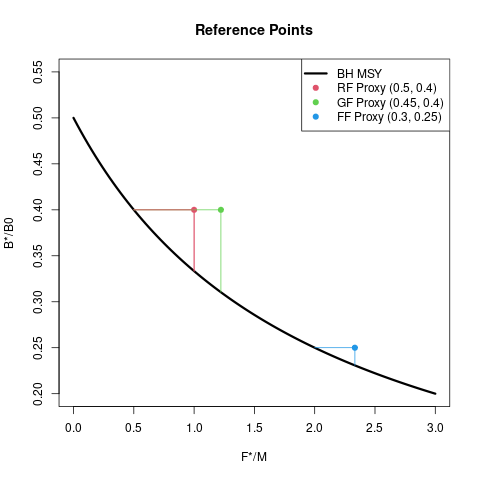
\includegraphics[width=\textwidth]{../gpBias/rpProxTable.png}
\end{minipage}
\end{figure}

%%
%\begin{table}
%\begin{tabular}{c|c|c|c|c|c}
%   & x    & $\frac{F_{SPR_x}}{M}$ & $\left[\frac{F_{MSY}(y)}{M}\right]_{BH}$ & $y \atop (\text{of }B_y)$ & $\left[\frac{\bar B(F_{SPR_x})}{B_0}\right]_{BH}$ \\ \hline %& $\left[F_{MSY}\right]_{BH}$\\ %$\left[\frac{F_{MSY}}{M}\right]_{BH} (F Only)$ \\ 
%RF & 0.50 & $1$			  & $1/2$ 				     & $2/5$  	 & 0.29 \\ %& 0.29\\ %1.45 (0.29)\\
%GF & 0.45 & $11/9$ 		  & $1/2$ 				     & $2/5$  	 & 0.22 \\ %& 0.49\\ %2.46 (0.49)\\
%FF & 0.30 & $7/3$		  & $2$ 				     & $1/4$  	 & 0.21 \\ %& 0.57   %2.87 (0.57)
%\end{tabular}
%\caption{ \label{proxyTable}
%Management targets and BH $\frac{B_{MSY}}{B_0}$ values for Rockfish, Groundfish, and Flatfish management categories.
%}
%\end{table}


%
In Figure (\ref{proxyTable}) notice that $y>\left[\frac{\bar B(F_{SPR_x})}{B_0}\right]_{BH}$ %\left[\frac{B_{MSY}}{B_0}\right]_{BH}$ 
consistently for all categories. This is a conservative management approach 
from the BH perspective since species are managed to biomasses %(thought to be)
that are greater than the BH $B^*$, but it also admits that proxy values 
are inconsistent with the underlying dynamics used to estimate biomass in 
the first place. Furthermore the BH SPM neccessitiates that the chosen proxy 
values will never equal the RPs they are intended to approximate.

%{\color{blue}
%\item Show BH calculation only hits target for $\frac{\alpha}{M}=6$; target cannot equal MSY.
%
%Consider the example of RF proxy values $B_{40}$ and $SPR_{50}$
%Satisfying the proxy values under the BH model 
%
%\item Show general $\alpha$-$\gamma$ proxy relation under Schnute.
%}



%%
%$B_0$ given by Eq. (\ref{B0S}). $R_0$ is given by evaluating $R(B_0; \theta)$.
%
%%
%\begin{equation}
%R_0 = \frac{M}{\gamma\beta} \left(1-\left(\frac{M}{\alpha}\right)^\gamma\right)
%\end{equation}
%
%%
%\begin{equation}
%F_{SPR_x} = \frac{R_0}{x B_0}-M = M\left(\frac{1}{x}-1\right)\label{fspr}
%\end{equation}

%
Under the three-parameter Schnute model the $\gamma$ parameter provides an 
additional degree of freedom that can be used to resolve the limiting 
issues presented by the BH model in any of a number of ways. 
%With informative indicies and global optimization one my estimate any (or both) of $\alpha$, $\beta$ and $\gamma$ 
%to calculate RP directly as seen in Section (\ref{}estimating more).
%Or 
One potentiallly compelling use of this extra degree of freedom is to  
%One may 
engineer the values of $\alpha$ and $\gamma$ to demand consistency of 
the proxies and $MSY$.
This necessitates that RPs are always equal to their measurable proxy approximations, 
and it resolves the inconsistency between proxies and the underlying dynamics 
used to estimate the biomasses to which they are compared. The Schnute model 
can do this by using $\gamma$ to tie proxies directly to the true RPs that 
they are intended to approximate. This makes proxies measurable quantities 
that truly represent the Schnute $MSY$ RPs. 
%ll while allowing some of the structure of the structure of productivity to be learned from data  
%Since under the Schnute model the 
%To derive the 

%
To derive the values of $\alpha$ and $\gamma$ that will result in consistency of
the proxies with $MSY$ we first consider the expression of $\frac{\bar B(F)}{B_0}$ 
under the Schnute SPM (similar to Eq.(\ref{BratS})) evaluated at $F_{SPR_x}$ (as given in Eq. (\ref{fspr})) %given in Eq.(\ref{BratS}). Enforcing that $F^*=F_{SPR_x}$ is as simple as replacing the 
%
\begin{align}
	\frac{\bar B(F_{SPR_x})}{B_0} &= \frac{1-\left(\frac{M+\left[M\left(\frac{1}{x}-1\right)\right]}{\alpha}\right)^\gamma}{ 1-\left(\frac{M}{\alpha}\right)^\gamma } \nonumber\\
	y&=\frac{1-\left(\frac{M}{x\alpha}\right)^\gamma}{ 1-\left(\frac{M}{\alpha}\right)^\gamma } \label{why}.
\end{align}

%Evaluating $\frac{B_{MSY}}{B_0}$ Eq.(\ref{BratS}) at $F_{SPR_x}$. 
Solving Eq. (\ref{why}) for $\alpha$ gives a relation between $\alpha$, 
and $\gamma$ that defines an infinite family of Schnute curves that 
respect the proxy values $x$ and $y$.
% the compensation ratio $\frac{\alpha}{M}$ gives,
%
\begin{equation}
\alpha = M\left[ \frac{\frac{1}{x^\gamma}-y}{1-y} \right]^{1/\gamma} \label{aProxy} %\frac{1}{\gamma}}
\end{equation}

%{\color{blue}
%\item Show general $\alpha$-$\gamma$ MSY relation under Schnute.\\
%}

%
Now to align the proxy $\alpha$-$\gamma$ values given by Eq. (\ref{aProxy}) 
with $MSY$ RPs we recall Eq.(\ref{abgSys}) from the text,
\begin{equation}
\alpha = (M+F^*)\left(1+\frac{\gamma F^*}{M+F^*}\right)^{1/\gamma}. \label{aMsy}
\end{equation}
While this expression for $\alpha$ was previously used in simulation design, 
here it is used as a relation between $\alpha$ and $\gamma$ that defines an 
infinite family of Schnute curves that respect a given value of $F^*$. 
Eqs. (\ref{aProxy}) and (\ref{aMsy}) each define different sub-families of 
Schnute curves that respect the proxies and $MSY$ respectively. When taken together,
the curves intersect to uniquely identify a single pair $(\alpha, \gamma)$ that
both respect the proxies and $MSY$ simultaneously. With the aim of isolating this point, 
%$(\alpha, \gamma)$ 
Eq. (\ref{aProxy}) and Eq. (\ref{aMsy}) can be equated to find the 
value of $\gamma$ that brings proxies into agreement with $MSY$. When RPs and 
proxies are in agreement, $F^*=F_{SPR_x}$ and thus $F^*$ in Eq. (\ref{aMsy})  
may be replaced by Eq. (\ref{fspr}) to write the $MSY$ relation in terms of $x$ and $y$ as, 
\begin{equation}
\alpha = \frac{M}{x}\Big(1+\gamma(1-x)\Big)^{1/\gamma} \label{aMSY}.
\end{equation}
 

%{\color{blue}
%Reference $\alpha$ Eq.(\ref{abgSys}) from text in $F_{MSY}$.\\
%When $F_{MSY}=F_{SPR_x}$ substitute in Eq.(\ref{fspr})
%\begin{equation}
%\frac{\alpha}{M} = \frac{1}{x}\Big(1+\gamma(1-x)\Big)^{1/\gamma} %\label{aMSY}
%\end{equation}
%\item Show single $(\alpha, \gamma)$ pair to hit both proxy and MSY.
%}

%
Now equating Eqs. (\ref{aProxy}) and (\ref{aMSY}) and then simplifying with the aim of solving for $\gamma$ gives,
%
\begin{align*}
\left[ \frac{\frac{1}{x^\gamma}-y}{1-y} \right]^{1/\gamma} &= \frac{1}{x}\Big(1+\gamma(1-x)\Big)^{1/\gamma}\\
1-yx^\gamma &= \Big(1+\gamma(1-x)\Big)(1-y)\\
1 &= \left[ 1-\gamma\frac{(1-x)(1-y)}{y}\right]x^{-\gamma}.
\end{align*}

%
At this point it convenient to make the substitution $r(x,y)=\frac{y}{(1-x)(1-y)}$. Making this substitution, and factoring, simplifies the form as,
%
\begin{align}
r(x,y)&=\Big(r(x,y)-\gamma\Big)x^{-\gamma}.
\end{align}

%
Recall the Lambert product logarithm, $W$, is defined as the inverse function of $x e^x$ such that $x=W(xe^x)$.
Isolating $\gamma$ requires that the above expression be placed into the form $xe^x$ to apply the definition of $W$. %the Applying this definition allows for the isolation of $\gamma$.
\begin{align}
r(x, y)x^{r(x, y)}&=\Big(r(x, y)-\gamma\Big)x^{r(x, y)-\gamma} \nonumber\\
r(x, y)x^{r(x, y)}\log(x) &= \Big(r(x, y)-\gamma\Big)\log(x) e^{\big(r(x, y)-\gamma\big)\log(x)} \nonumber\\
W_{-1}\Big(r(x, y)x^{r(x, y)}\log(x)\Big) &= \Big(r(x, y)-\gamma\Big)\log(x) \nonumber\\
\gamma &= r(x, y)-\frac{W_{-1}\Big(r(x, y)x^{r(x, y)}\log(x)\Big)}{\log(x)} \label{gOfProxy}
\end{align}
%
The solution of interest for the $\gamma$, that brings the proxies into agreement 
with MSY, comes from $W_{-1}$.
%
To complete the point $(\alpha, \gamma)$, $\alpha$ may be computed by 
substituting $\gamma$ from Eq. (\ref{gOfProxy}) into either of 
Eqs. (\ref{aProxy}) or (\ref{aMSY}) to give $\alpha$ in terms of only the proxies and the Lambert product logarithm. 

%\clearpage
\begin{wrapfigure}{r}{0.49\textwidth}
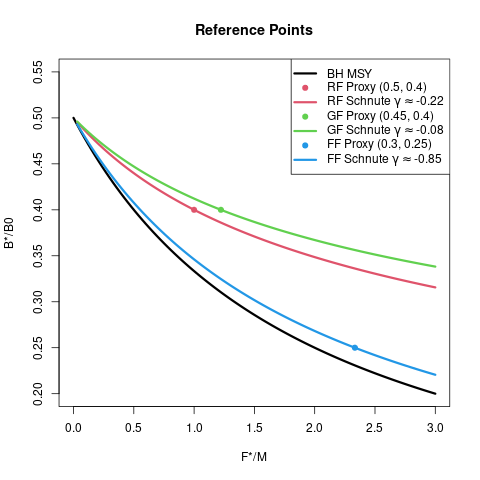
\includegraphics[width=0.49\textwidth]{../gpBias/rpProxAll0.2.png}
\caption{\label{rpProxCurves}BH MSY RP curve, along side Schnute MSY RP curves with $\gamma$ chosen to match the management proxies.}
\end{wrapfigure}
%
Figure (\ref{rpProxCurves}) demonstrates how the BH RPs can be generalized by 
the three parameter Schnute model to bring $MSY$ RPs into alignment with the 
proxy values. The colored curves show the RPs that a Schnute model with 
$\gamma$'s fixed by Eq. (\ref{gOfProxy}) can model. Notice that the proxy values 
fall along the colored curves, with the specific location of the the proxy point 
given by the $\alpha$ derived by plugging $\gamma$ back into either of Eqs. (\ref{aProxy}) 
or (\ref{aMSY}).

%
%In concept other three parameter model should allow similar flexibility
In concept, other three-parameter models should allow similar flexibility, but 
the results may not be analytical as given here for the Schnute model. While 
other three-parameter models should be able to bring RPs into correspondence 
with their proxies, the differing functional forms of various three-parameter 
models may result in yield curves that behave in unexpected ways. A beautiful 
feature of the Schnute model used in this way is that the derived $\gamma$ 
values generalize the BH model in a way that results in familiar yield curves 
such as the Cushing, BH, Ricker, or Logistic models with well studied risk 
characteristics. 
%(or interpolation between those models)

%which is that have may result in more or less conservative resolutions of their parametric forms and RPs. 
%f various

%\end{itemize}
